\section{General}
\includecpp{C++ Template}{"./src/1.general/01.c++-template.cpp"}
\includecpp{Troubleshoot}{"./src/1.general/02.troubleshoot.cpp"}
\section{Data Structures}
\includecpp{Disjoin Set Union}{"./src/2.data-structures/01.disjoin-set-union.cpp"}
\includecpp{Fenwick Tree Point Update And Range Query}{"./src/2.data-structures/02.fenwick-tree-point-update-and-range-query.cpp"}
\includecpp{Fenwick Tree Range Update And Point Query}{"./src/2.data-structures/03.fenwick-tree-range-update-and-point-query.cpp"}
\includecpp{Fenwick Tree Range Update And Range Query}{"./src/2.data-structures/04.fenwick-tree-range-update-and-range-query.cpp"}
\includecpp{Fenwick 2D}{"./src/2.data-structures/05.fenwick-2D.cpp"}
\includecpp{Segment Tree}{"./src/2.data-structures/06.segment-tree.cpp"}
\includecpp{Treap}{"./src/2.data-structures/07.treap.cpp"}
\section{Graphs}
\includecpp{Floyd}{"./src/3.graphs/1.floyd.cpp"}
\includecpp{Bridges}{"./src/3.graphs/10.bridges.cpp"}
\includecpp{Cut Points}{"./src/3.graphs/11.cut-points.cpp"}
\includecpp{Condense}{"./src/3.graphs/12.condense.cpp"}
\includetex{Number Of Paths Of Fixed Length}{"./src/3.graphs/13.number-of-paths-of-fixed-length.texs"}
\includetex{Shortest Paths Of Fixed Length}{"./src/3.graphs/14.shortest-paths-of-fixed-length.texs"}
\includecpp{Dijkstra}{"./src/3.graphs/2.dijkstra.cpp"}
\includecpp{Bellmanford}{"./src/3.graphs/3.bellmanford.cpp"}
\includecpp{Kruskal}{"./src/3.graphs/4.kruskal.cpp"}
\includecpp{Topo Sort}{"./src/3.graphs/5.topo-sort.cpp"}
\includecpp{Khun}{"./src/3.graphs/6.khun.cpp"}
\includecpp{Khun Ex}{"./src/3.graphs/7.khun-ex.cpp"}
\includecpp{Lca}{"./src/3.graphs/8.lca.cpp"}
\includecpp{Bipartite Checking}{"./src/3.graphs/9.bipartite-checking.cpp"}
\section{Math}
\includecpp{Linear Sieve}{"./src/4.math/01.linear-sieve.cpp"}
\includecpp{Extended Euclidean Algorithm}{"./src/4.math/02.extended-euclidean-algorithm.cpp"}
All other solutions can be found like this:
$$x' = x - k \frac{b}{g}, y' = y + k \frac{a}{g}, k \in \mathbb{Z}$$
\includetex{Chinese Remainder Theorem}{"./src/4.math/04.chinese-remainder-theorem.texs"}
\includecpp{Euler Totient Function}{"./src/4.math/05.euler-totient-function.cpp"}
\includecpp{Factorization With Sieve}{"./src/4.math/06.factorization-with-sieve.cpp"}
\includecpp{Modular Inverse}{"./src/4.math/07.modular-inverse.cpp"}
\includecpp{Simpson Integration}{"./src/4.math/08.simpson-integration.cpp"}
\includetex{Burnside's Lemma}{"./src/4.math/09.burnside's-lemma.texs"}
\includecpp{FFT}{"./src/4.math/10.FFT.cpp"}
\includecpp{FFT With Modulo}{"./src/4.math/11.FFT-with-modulo.cpp"}
\includecpp{Big Integer Multiplication With FFT}{"./src/4.math/12.big-integer-multiplication-with-FFT.cpp"}
\includecpp{Gaussian Elimination}{"./src/4.math/13.gaussian-elimination.cpp"}
\includetex{Sprague Grundy Theorem}{"./src/4.math/14.sprague-grundy-theorem.texs"}
\includetex{Formulas}{"./src/4.math/99.formulas.texs"}
\section{Geometry}
\includecpp{2d Vector}{"./src/5.geometry/01.2d-vector.cpp"}
\includecpp{Line}{"./src/5.geometry/02.line.cpp"}
\includecpp{Convex Hull Gift Wrapping}{"./src/5.geometry/03.convex-hull-gift-wrapping.cpp"}
\includecpp{Convex Hull With Graham's Scan}{"./src/5.geometry/04.convex-hull-with-graham's-scan.cpp"}
\includecpp{Circle Line Intersection}{"./src/5.geometry/05.circle-line-intersection.cpp"}
\includetex{Circle Circle Intersection}{"./src/5.geometry/06.circle-circle-intersection.texs"}
\includecpp{Common Tangents To Two Circles}{"./src/5.geometry/07.common-tangents-to-two-circles.cpp"}
\includetex{Number Of Lattice Points On Segment}{"./src/5.geometry/08.number-of-lattice-points-on-segment.texs"}
\includetex{Pick's Theorem}{"./src/5.geometry/09.pick's-theorem.texs"}
\includecpp{Usage Of Complex}{"./src/5.geometry/98.usage-of-complex.cpp"}
\includetex{Misc}{"./src/5.geometry/99.misc.texs"}
\section{Strings}
\includecpp{Hashing}{"./src/6.strings/01.hashing.cpp"}
\includecpp{Prefix Function}{"./src/6.strings/02.prefix-function.cpp"}
\includecpp{Prefix Function Automaton}{"./src/6.strings/03.prefix-function-automaton.cpp"}
\includecpp{KMP}{"./src/6.strings/04.KMP.cpp"}
\includecpp{Aho Corasick Automaton}{"./src/6.strings/05.aho-corasick-automaton.cpp"}
\includecpp{Suffix Array}{"./src/6.strings/06.suffix-array.cpp"}
\section{Dynamic Programming}
\includecpp{Convex Hull Trick}{"./src/7.dynamic-programming/01.convex-hull-trick.cpp"}
\includecpp{Divide And Conquer}{"./src/7.dynamic-programming/02.divide-and-conquer.cpp"}
\includetex{Optimizations}{"./src/7.dynamic-programming/99.optimizations.texs"}
\section{Misc}
\includetex{Mo's Algorithm}{"./src/8.misc/01.mo's-algorithm.texs"}
\includecpp{Ternary Search}{"./src/8.misc/02.ternary-search.cpp"}
\includecpp{Big Integer}{"./src/8.misc/03.big-integer.cpp"}
\includecpp{Binary Exponentiation}{"./src/8.misc/04.binary-exponentiation.cpp"}
\includetex{Builtin GCC Stuff}{"./src/8.misc/99.builtin-GCC-stuff.texs"}

% Written by Anders Sjoqvist and Ulf Lundstrom, 2009
% The main sources are: tinyKACTL, Beta and Wikipedia

\section{Mathematics}

\subsubsection{Equations}
\[ax^2+bx+c=0 \Rightarrow x = \frac{-b\pm\sqrt{b^2-4ac}}{2a}\]

The extremum is given by $x = -b/2a$.

\[\begin{aligned}ax+by=e\\cx+dy=f\end{aligned}
\Rightarrow
\begin{aligned}x=\dfrac{ed-bf}{ad-bc}\\y=\dfrac{af-ec}{ad-bc}\end{aligned}\]

In general, given an equation $Ax = b$, the solution to a variable $x_i$ is given by
\[x_i = \frac{\det A_i'}{\det A} \]
where $A_i'$ is $A$ with the $i$'th column replaced by $b$.

\subsubsection{Recurrences}
If $a_n = c_1 a_{n-1} + \dots + c_k a_{n-k}$, and $r_1, \dots, r_k$ are distinct roots of $x^k + c_1 x^{k-1} + \dots + c_k$, there are $d_1, \dots, d_k$ s.t.
\[a_n = d_1r_1^n + \dots + d_kr_k^n. \]
Non-distinct roots $r$ become polynomial factors, e.g. $a_n = (d_1n + d_2)r^n$.

\subsubsection{Trigonometry}
\begin{align*}
\sin(v+w)&{}=\sin v\cos w+\cos v\sin w\\
cos(v+w)&{}=\cos v\cos w-\sin v\sin w\\
\end{align*}
\begin{align*}
\tan(v+w)&{}=\dfrac{\tan v+\tan w}{1-\tan v\tan w}\\
\sin v+\sin w&{}=2\sin\dfrac{v+w}{2}\cos\dfrac{v-w}{2}\\
\cos v+\cos w&{}=2\cos\dfrac{v+w}{2}\cos\dfrac{v-w}{2}
\end{align*}
\[ (V+W)\tan(v-w)/2{}=(V-W)\tan(v+w)/2 \]
where $V, W$ are lengths of sides opposite angles $v, w$.
\begin{align*}
	a\cos x+b\sin x&=r\cos(x-\phi)\\
	a\sin x+b\cos x&=r\sin(x+\phi)
\end{align*}
where $r=\sqrt{a^2+b^2}, \phi=\operatorname{atan2}(b,a)$.

\subsubsection{Geometry}

\subsection{Triangles}
Side lengths: $a,b,c$\\
Semiperimeter: $p=\dfrac{a+b+c}{2}$\\
Area: $A=\sqrt{p(p-a)(p-b)(p-c)}$\\
Circumradius: $R=\dfrac{abc}{4A}$\\
Inradius: $r=\dfrac{A}{p}$\\
Length of median (divides triangle into two equal-area triangles): $m_a=\tfrac{1}{2}\sqrt{2b^2+2c^2-a^2}$\\
Length of bisector (divides angles in two): $s_a=\sqrt{bc\left[1-\left(\dfrac{a}{b+c}\right)^2\right]}$\\
Law of sines: $\dfrac{\sin\alpha}{a}=\dfrac{\sin\beta}{b}=\dfrac{\sin\gamma}{c}=\dfrac{1}{2R}$\\
Law of cosines: $a^2=b^2+c^2-2bc\cos\alpha$\\
Law of tangents: $\dfrac{a+b}{a-b}=\dfrac{\tan\dfrac{\alpha+\beta}{2}}{\tan\dfrac{\alpha-\beta}{2}}$\\

\subsection{Quadrilaterals}
With side lengths $a,b,c,d$, diagonals $e, f$, diagonals angle $\theta$, area $A$ and
magic flux $F=b^2+d^2-a^2-c^2$:

\[ 4A = 2ef \cdot \sin\theta = F\tan\theta = \sqrt{4e^2f^2-F^2} \]

 For cyclic quadrilaterals the sum of opposite angles is $180^\circ$,
$ef = ac + bd$, and $A = \sqrt{(p-a)(p-b)(p-c)(p-d)}$.

\subsection{Spherical coordinates}
\centerline{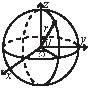
\includegraphics[width=50mm]{src/9.kactl/sphericalCoordinates.pdf}}
\[\begin{array}{cc}
x = r\sin\theta\cos\phi & r = \sqrt{x^2+y^2+z^2}\\
y = r\sin\theta\sin\phi & \theta = \textrm{acos}(z/\sqrt{x^2+y^2+z^2})\\
z = r\cos\theta & \phi = \textrm{atan2}(y,x)
\end{array}\]

\subsubsection{Derivatives/Integrals}
\begin{align*}
	\dfrac{d}{dx}\arcsin x = \dfrac{1}{\sqrt{1-x^2}} &&& \dfrac{d}{dx}\arccos x = -\dfrac{1}{\sqrt{1-x^2}} \\
	\dfrac{d}{dx}\tan x = 1+\tan^2 x &&& \dfrac{d}{dx}\arctan x = \dfrac{1}{1+x^2} \\
	\int\tan ax = -\dfrac{\ln|\cos ax|}{a} &&& \int x\sin ax = \dfrac{\sin ax-ax \cos ax}{a^2} \\
	\int e^{-x^2} = \frac{\sqrt \pi}{2} \text{erf}(x) &&& \int xe^{ax}dx = \frac{e^{ax}}{a^2}(ax-1)
\end{align*}

Integration by parts:
\[\int_a^bf(x)g(x)dx = [F(x)g(x)]_a^b-\int_a^bF(x)g'(x)dx\]

\subsubsection{Sums}
\[ c^a + c^{a+1} + \dots + c^{b} = \frac{c^{b+1} - c^a}{c-1}, c \neq 1 \]
\begin{align*}
	1 + 2 + 3 + \dots + n &= \frac{n(n+1)}{2} \\
	1^2 + 2^2 + 3^2 + \dots + n^2 &= \frac{n(2n+1)(n+1)}{6} \\
	1^3 + 2^3 + 3^3 + \dots + n^3 &= \frac{n^2(n+1)^2}{4} \\
	1^4 + 2^4 + 3^4 + \dots + n^4 &= \frac{n(n+1)(2n+1)(3n^2 + 3n - 1)}{30} \\
\end{align*}

\subsubsection{Series} 
$$e^x = 1+x+\frac{x^2}{2!}+\frac{x^3}{3!}+\dots,\,(-\infty<x<\infty)$$
$$\ln(1+x) = x-\frac{x^2}{2}+\frac{x^3}{3}-\frac{x^4}{4}+\dots,\,(-1<x\leq1)$$
$$\sqrt{1+x} = 1+\frac{x}{2}-\frac{x^2}{8}+\frac{2x^3}{32}-\frac{5x^4}{128}+\dots,\,(-1\leq x\leq1)$$
$$\sin x = x-\frac{x^3}{3!}+\frac{x^5}{5!}-\frac{x^7}{7!}+\dots,\,(-\infty<x<\infty)$$
$$\cos x = 1-\frac{x^2}{2!}+\frac{x^4}{4!}-\frac{x^6}{6!}+\dots,\,(-\infty<x<\infty)$$